\chapter{Results} \label{ch:results}
Present results and comparisons to Adare et al.....

	\begin{figure}[h]
	  \centering
	  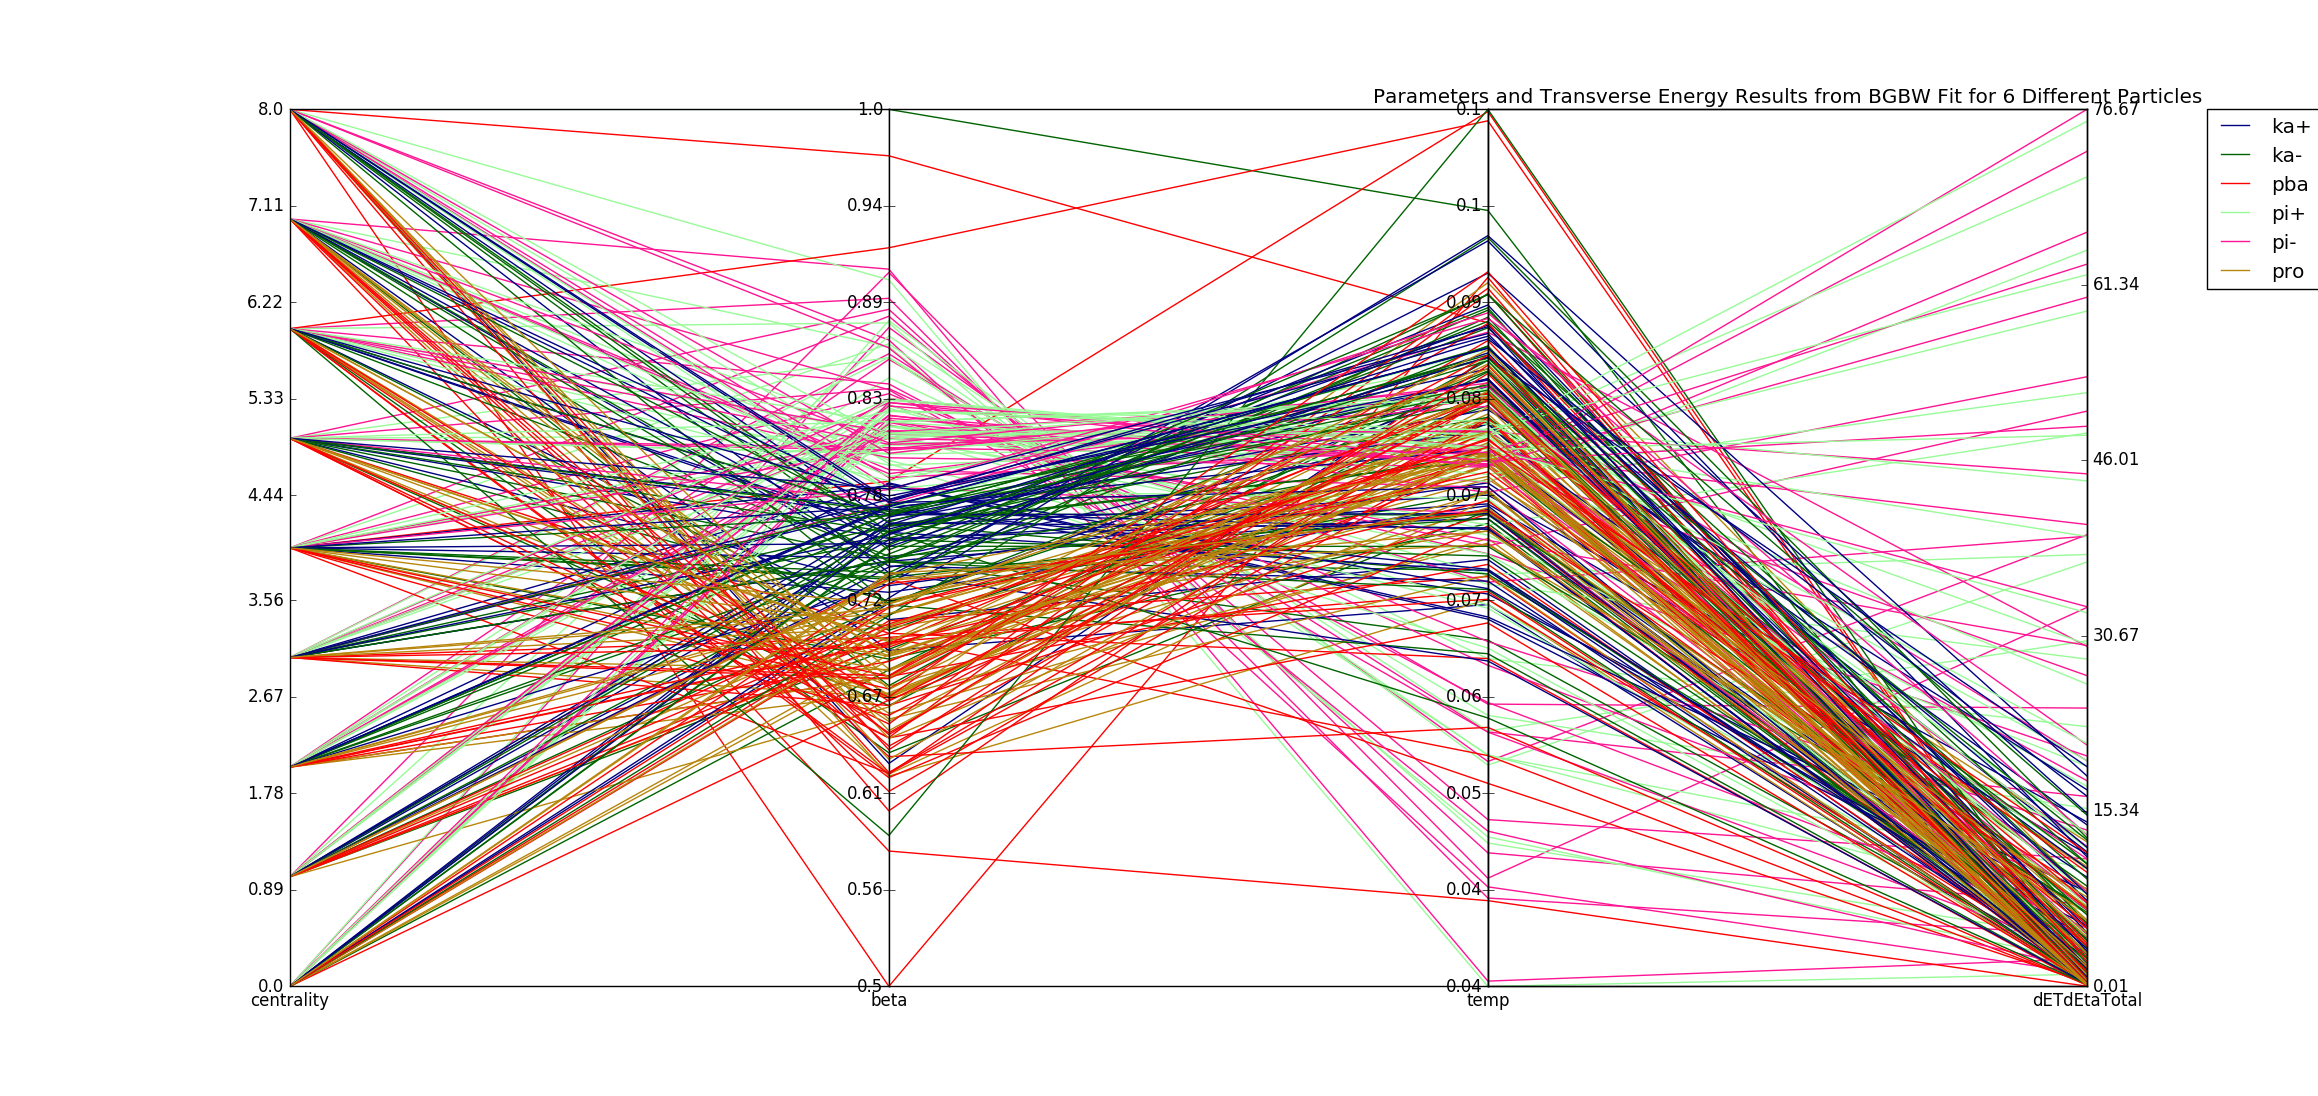
\includegraphics[width=6.5in]{figures/parallelCoordPlot_4Axes.png}
	  \caption{Parallel coordinates plot for 270 diffrent spectra relating 6 different identified particles (color-coded) to their respective collision centrality classes, good-fit parameters, and the transverse energy calculated using said parameters.}\label{fig:parallelCoord}
	\end{figure}
	
% cross-check plots: pseudorapidity
%%%%%%%%%%%%%%%%%%%%%%%%%%%%%%%%%%%%%%%%%%%%%%%%%%%%%%
	\begin{figure}[h]
	  \centering
	  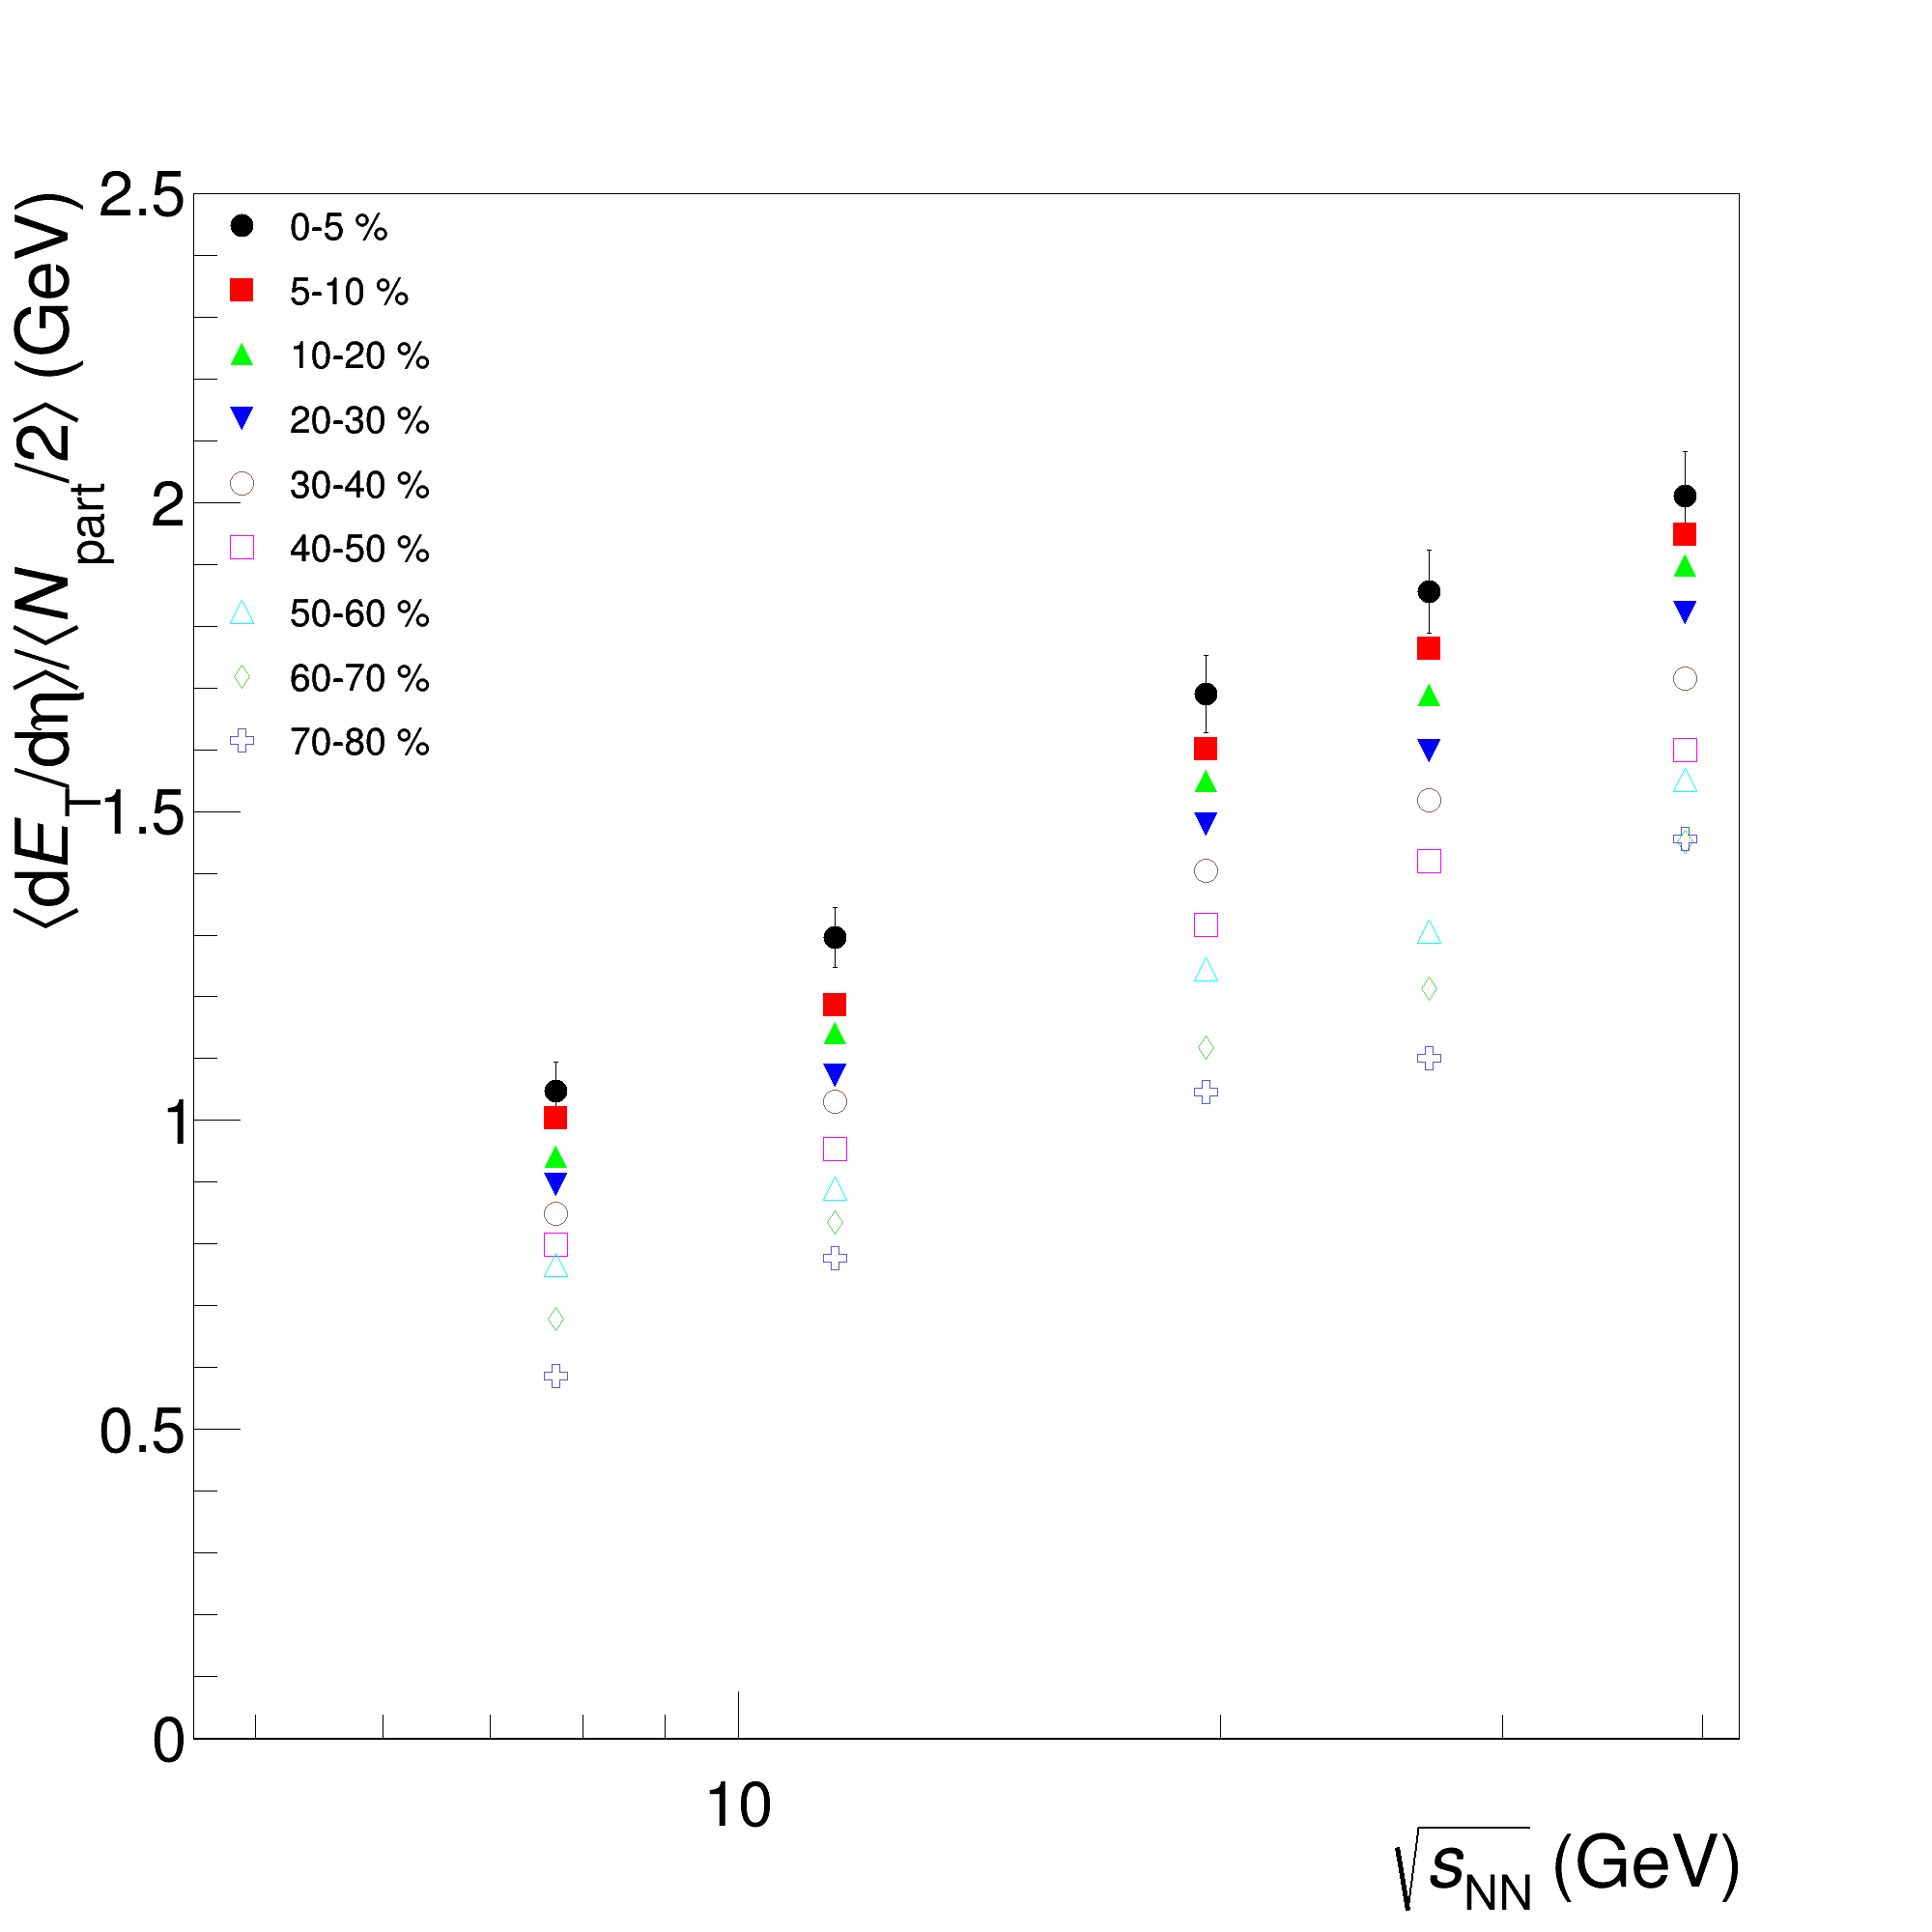
\includegraphics[width=5.5in]{figures/finalStacked/dETdEtaOverNpartBy2SumCent8s.png}
	  \caption{$(dE_{T}/d\eta)/0.5N_{part}$ at midrapidity as a function of $\sqrt{s_{NN}}$ for different centralities. The dashed line represents a power-law fit to the 0-5\% central data in the form $y = ax^{2b}$, where $x$ and $y$ are the placeholders for the quantities in the plot axes. $\chi^{2}/n.d.f$ for the fit was 1.806, and the good-fit parameters were $a = 0.4838 \pm 0.0429$ and $b = 0.2005 \pm 0.01466$. The shaded area represents the uncertainty bounds for the 0-5\% central PHENIX data from \cite{PhysRevC.93.024901}. }\label{fig:dETdEtaOverNpartBy2SumCents}
	\end{figure}
	
	\begin{figure}[h]
	  \centering
	  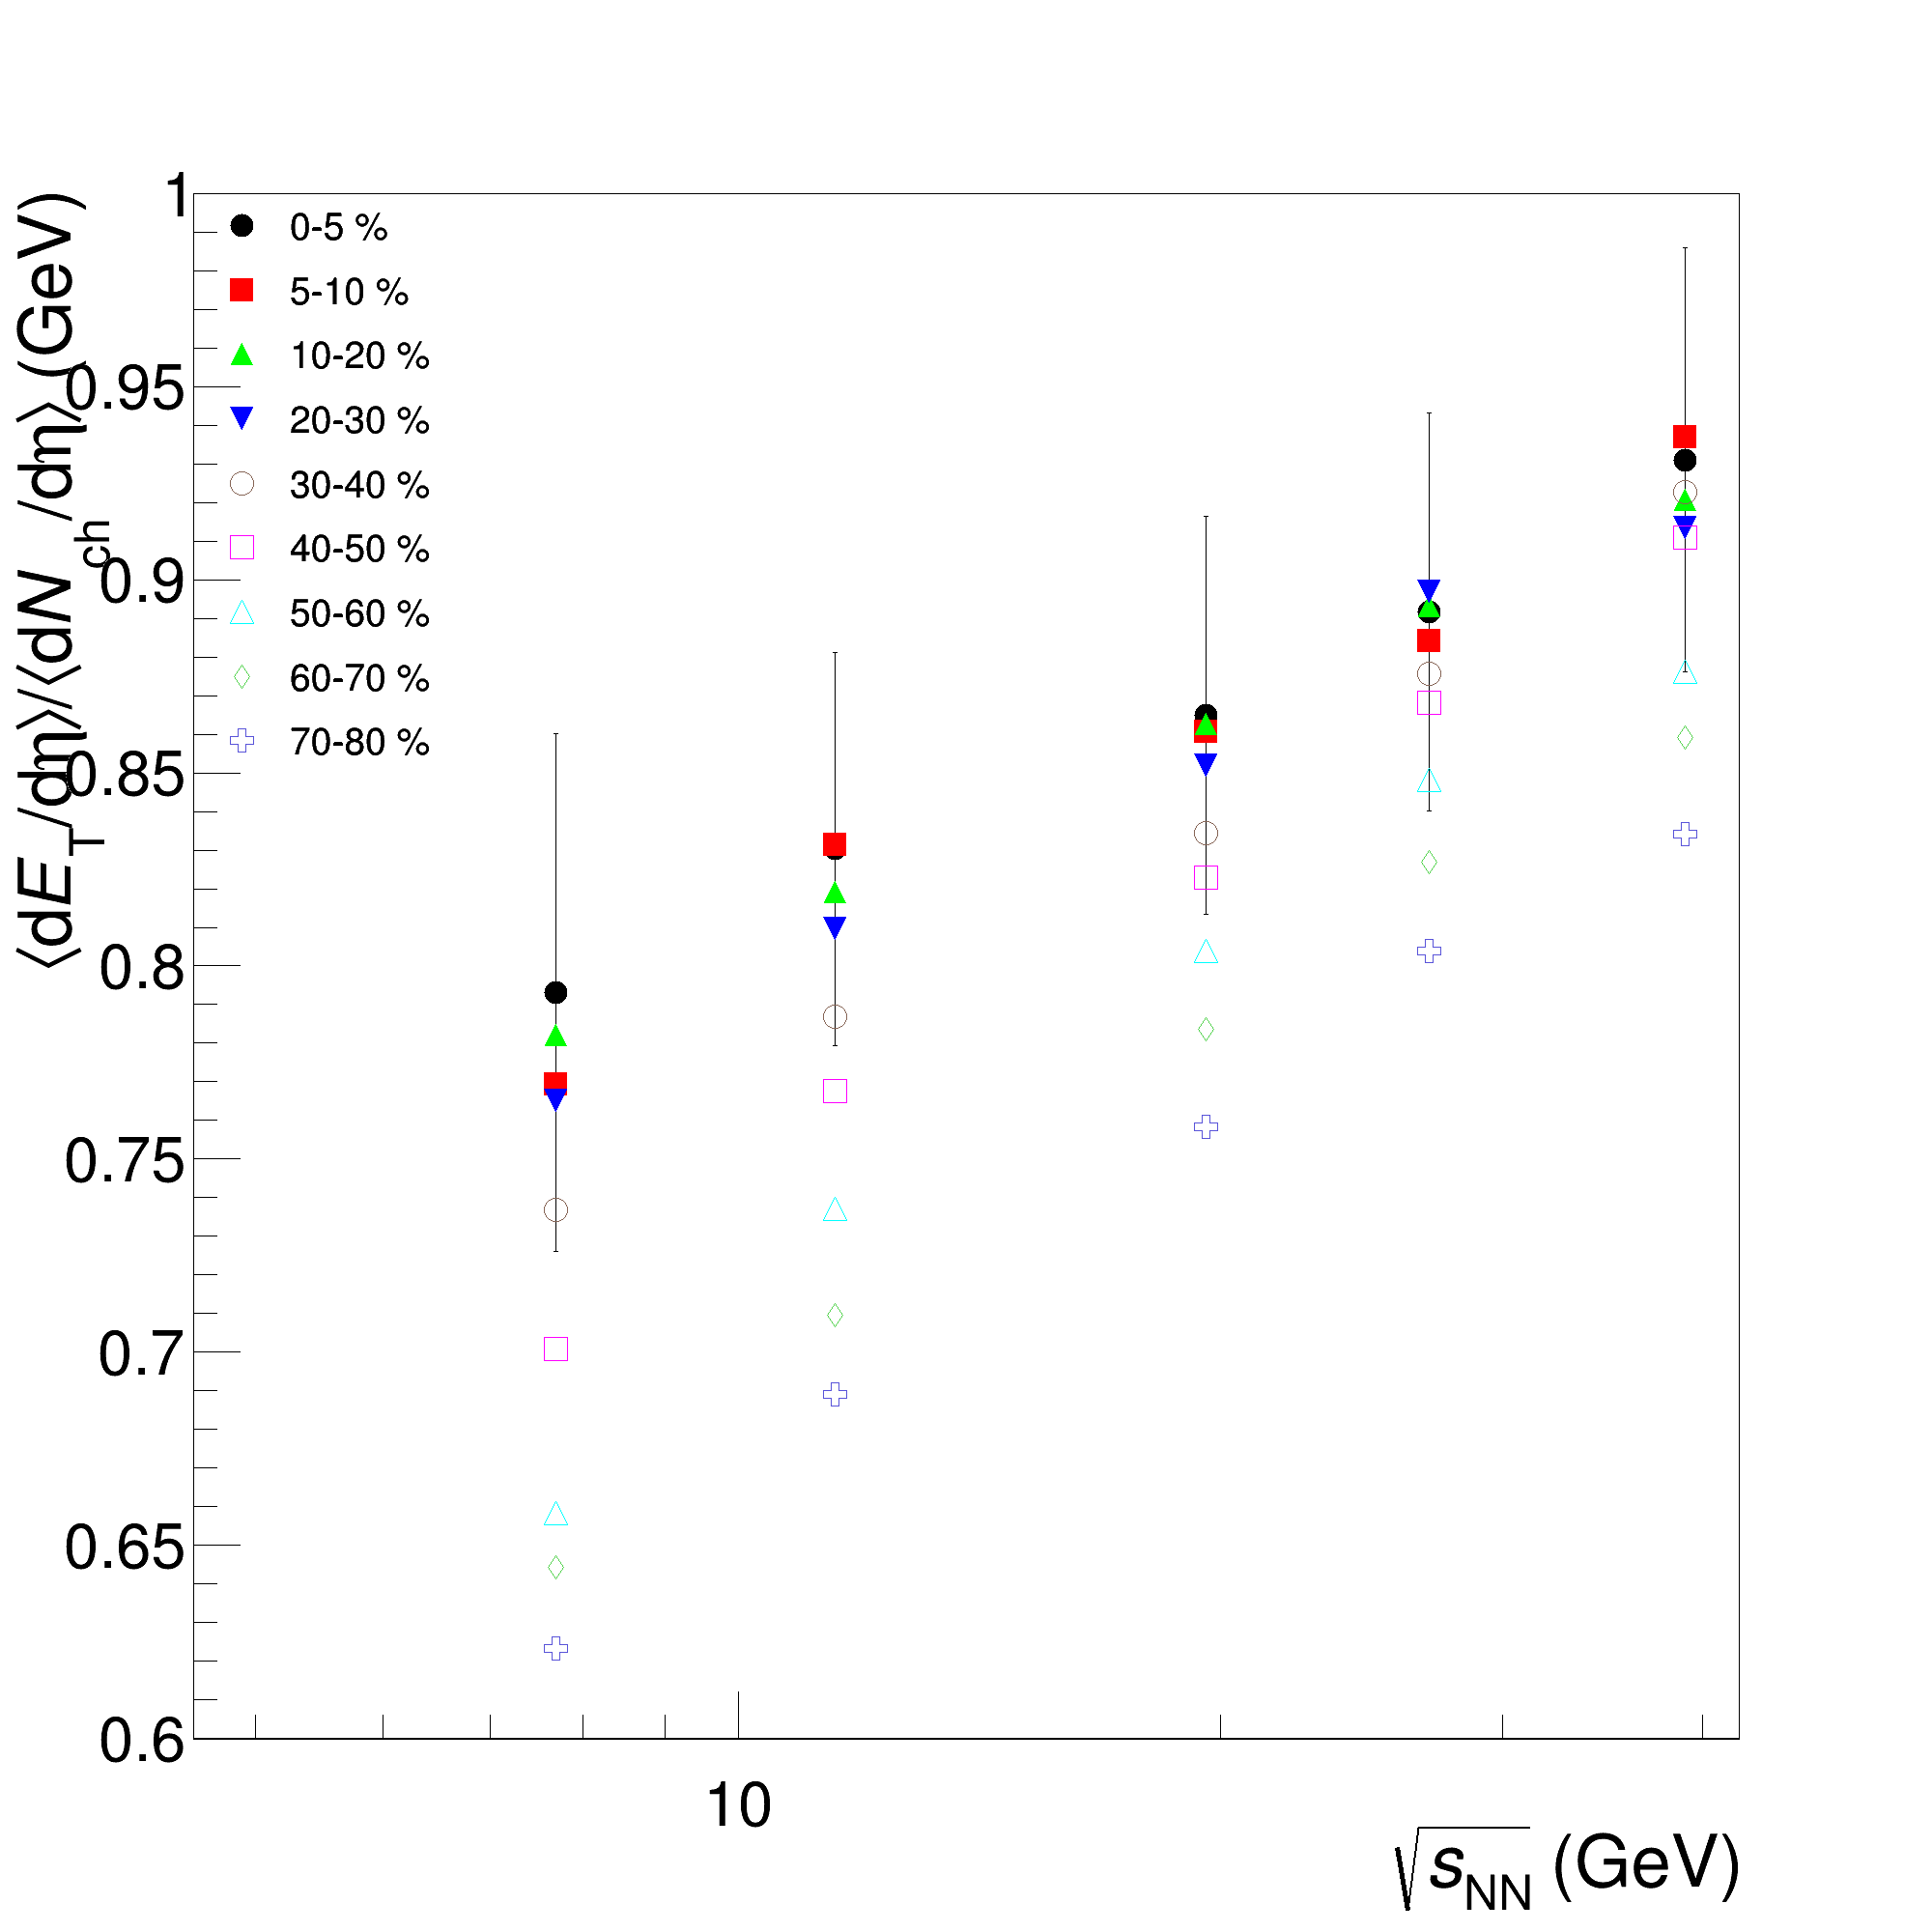
\includegraphics[width=5.5in]{figures/finalStacked/dETdEtaOverdNchdEtaSumCent8s.png}
	  \caption{$(dE_{T}/d\eta)/(dN_{ch}/d\eta)$ at midrapidity as a function of $\sqrt{s_{NN}}$ for different centralities.}\label{fig:dETdEtaOverdNchdEtaSumCents}
	\end{figure}
	
	\begin{figure}[h]
	  \centering
	  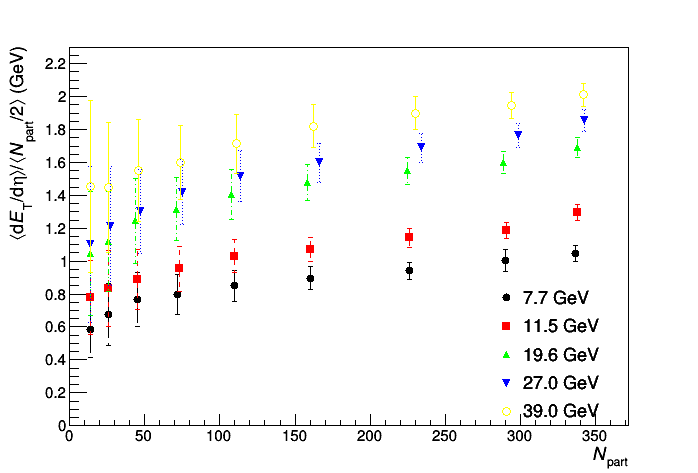
\includegraphics[width=5.5in]{{figures/finalStacked/dETdEtaOverNpartBy2SumEn39.0s}.png}
	  \caption{$(dE_{T}/d\eta)/0.5N_{part}$ at midrapidity as a function of ${N_{part}}$ for different centralities.}\label{fig:dETdEtaOverNpartBy2SumEn}
	\end{figure}
	
	\begin{figure}[h]
	  \centering
	  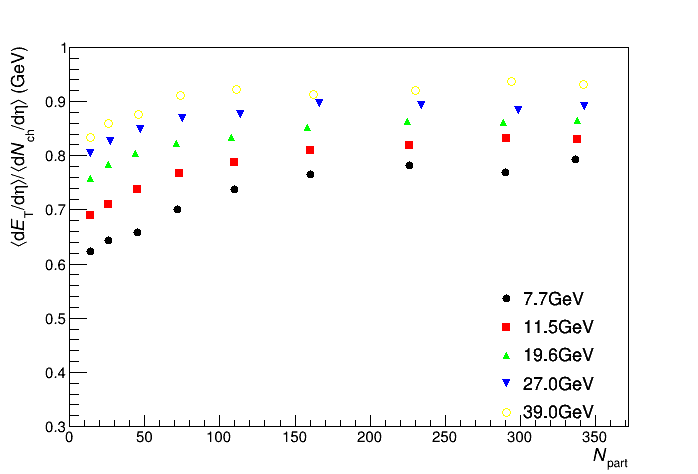
\includegraphics[width=5.5in]{{figures/finalStacked/dETdEtaOverdNchdEtaSumEn39.0s}.png}
	  \caption{$(dE_{T}/d\eta)/(dN_{ch}/d\eta)$ at midrapidity as a function of ${N_{part}}$ for different centralities.}\label{fig:dETdEtaOverdNchdEtaSumEn}
	\end{figure}

% cross-check plots: rapidity
%%%%%%%%%%%%%%%%%%%%%%%%%%%%%%%%%%%%%%%%%%%%%%%%%%%%%%
	\begin{figure}[h]
	  \centering
	  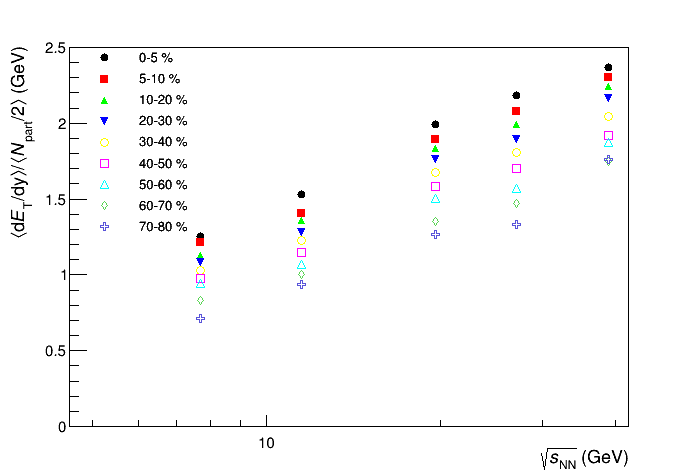
\includegraphics[width=5.5in]{figures/finalStacked/dETdyOverNpartBy2SumCent8s.png}
	  \caption{$(dE_{T}/dy)/0.5N_{part}$ at midrapidity as a function of $\sqrt{s_{NN}}$ for different centralities.}\label{fig:dETdyOverNpartBy2SumCents}
	\end{figure}
	
	\begin{figure}[h]
	  \centering
	  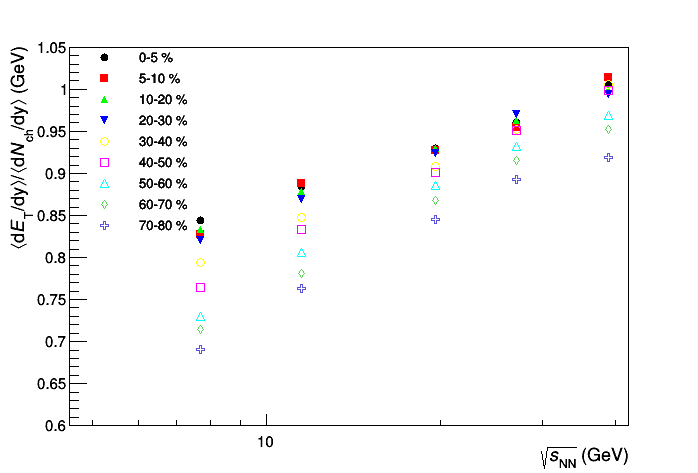
\includegraphics[width=5.5in]{figures/finalStacked/dETdyOverdNchdySumCent8s.png}
	  \caption{$(dE_{T}/dy)/(dN_{ch}/dy)$ at midrapidity as a function of $\sqrt{s_{NN}}$ for different centralities.}\label{fig:dETdyOverdNchdySumCents}
	\end{figure}
	
	\begin{figure}[h]
	  \centering
	  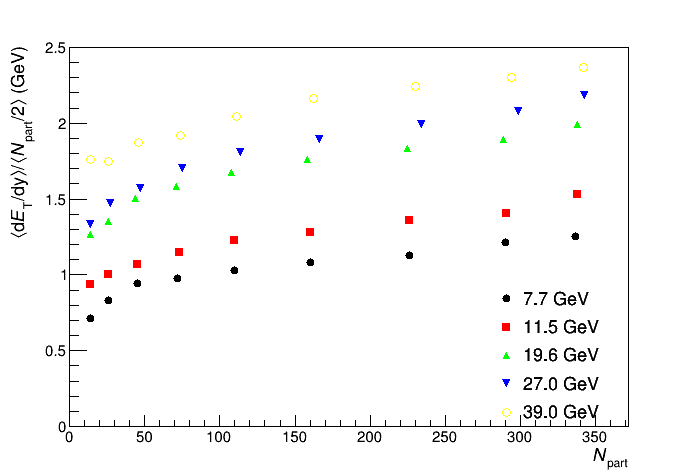
\includegraphics[width=5.5in]{{figures/finalStacked/dETdyOverNpartBy2SumEn39.0s}.png}
	  \caption{$(dE_{T}/dy)/0.5N_{part}$ at midrapidity as a function of ${N_{part}}$ for different centralities.}\label{fig:dETdyOverNpartBy2SumEn}
	\end{figure}
	
	\begin{figure}[h]
	  \centering
	  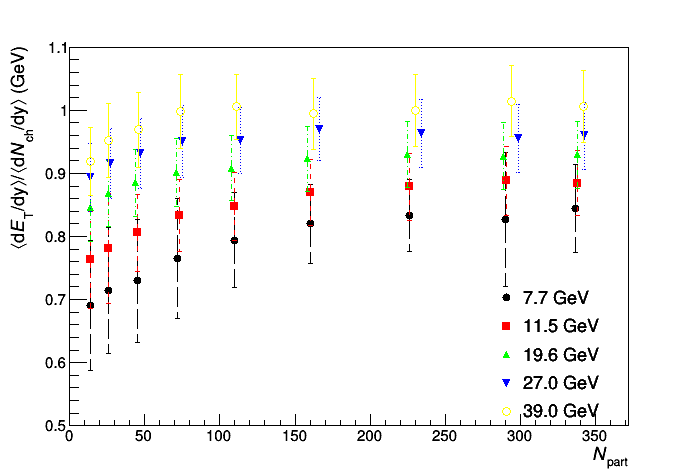
\includegraphics[width=5.5in]{{figures/finalStacked/dETdyOverdNchdySumEn39.0s}.png}
	  \caption{$(dE_{T}/dy)/(dN_{ch}/dy)$ at midrapidity as a function of ${N_{part}}$ for different centralities.}\label{fig:dETdyOverdNchdySumEn}
	\end{figure}

% comparison with Adare et al.
	\begin{figure}[h]
	  \centering
	  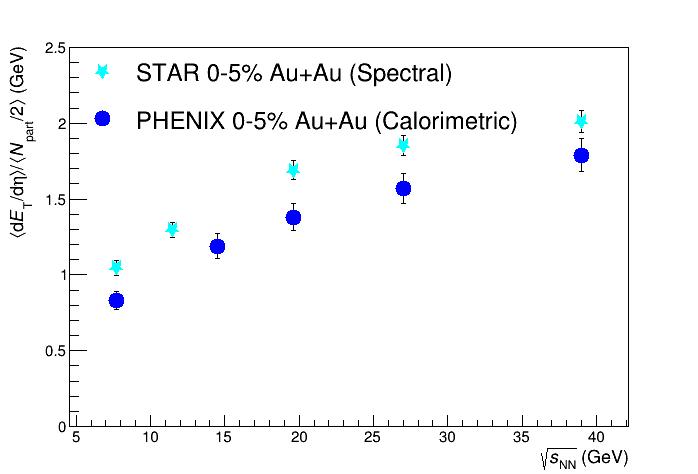
\includegraphics[width=4.5in]{figures/PHENIX_comparison2.png}
	  \caption{$\frac{dE_{T}}{d\eta}/0.5N_{part}$ for 0-5\% central collisions at midrapidity as a function of $\sqrt{s_{NN}}$. The PHENIX data are from \cite{PhysRevC.93.024901}. The error bars represent the total statistical and systematic uncertainties.}\label{fig:comparison}
	\end{figure}
	
	
	
%cnt97kx Send this link to your invitees ... http://whenisgood.net/fndqz2a This is where your results will appear ... http://whenisgood.net/fndqz2a/results/cnt97kx And use this link to edit your event ... http://whenisgood.net/fndqz2a/edit/cnt97kx
